% $Id: introduction.tex 87303 2016-02-08 13:44:29Z lafferty $
\clearpage
\newpage
\section{Appendix: Selection and BDT}
\label{app:selection}
%{\it Fill in the details of the stripping selection, fiducial cuts
%and BDT (RoC curves, signal and backgroung histrograms of input variables ...)}

% Stripping selections

The stripping selection lines for the \KsPzMuMu and \Kspipi candidates are
\begin{itemize}
 \item StrippingK0s2Pi0MuMuLines: used for the FULL \KsPzMuMu category
 \item TriggerTestLine (in StrippingRareNStrange): used for the PARTIAL \KsPzMuMu category.
\end{itemize}
Both stripping lines use the same selection criteria for \Kspipi. 
%  \item
%  \item
%  \item Daughters must not be compatible with coming directly from the PV, by requiring a high impact parameter $\chi^2$, which is defined as the difference of the $\chi^2$ of the PV fit obtained with and without 
%  the considered track.
The stripping criteria for all lines are summarized in \tabref{stripping:pipi}. They are as follows:
\begin{itemize}
 \item The \Kspipi sample is prescaled by a factor of 0.001 due to its large size.
 \item The charged-particle containers StdAllLooseMuons and StdNoPidsPions are used.
 \item Only resolved $\pi^{0}$ candidates are used, as the merged contribute only with additional 2.9\%.
 \item \KS{}  M: \KS\ candidate mass is required to be in the range [400, 600] \mevcc{} for the FULL and \Kspipi samples.
 \item $\mu^{+}\mu^{-}$  M: The dimuon candidate mass for the PARTIAL sample is required to be smaller than 450 \mevcc to reduce the contribution from misidentified \Kspipi. This is a loose requirement,
       given that the maximum dimuon mass, without considering the detector response, is $m_{\KS}-m_{\pi^{0}}=362$ \mevcc.
 \item \KS{} tof: Proper decay time of the \KS\ candidate given in a fraction of the \KS\ lifetime. This variable is computed using the reconstructed momentum of the \KS candidate and the distance between 
      the reconstructed secondary (SV) and primary (PV) vertices.
 \item \KS{} IP:  The \KS\ candidate must be compatible with the PV, asking for a low impact parameter with respect to PV.
 \item $\mu^{+}\mu^{-}$ DIRA: Forward \KS\ decay, requiring a positive cosine of the polar direction angle (DIRA).
 \item $\mu^{+}\mu^{-}$ DOCA: Good reconstruction quality of the SV required asking for a low distance of closest approach (DOCA) of the two daughter tracks.
 \item Daug. Track $\chi^{2}/ndof$:  Good reconstruction quality of the muon/pion tracks is required using the $\chi^{2}/ndof$ of the track fit. This is the standard cut of long tracks in LHCb.

 \item Daug. IP$_{\chi^{2}}$ : Daughters must not be compatible with coming directly from the PV, by requiring a high impact parameter $\chi^{2}$, which is defined as the difference of the $\chi^{2}$ of the PV
       fit obtained with and without the considered track.
 \item Daug. Track ghost prob.:  accounts for the probability that a track does not correspond to a track from a single charged particle.
 \item Daug. PID: The DLL $\mu-\pi$ ($log(P_{\mu}/P_{pi})$) is used to increase the muon purity at stripping level.
 \item Vertex $\rho$: The radial distance between the dimuon vertex in LHCb coordinates.
 \item Vertex $z$: The distance in $z$ (LHCb coordinates).
 \item Vertex $\chi^{2}/ndof$: A good-quality vertex is assured by placing a requirement on its fit quality.
 \item $\delta_{z}$: Distance from the end vertex of the particle and the related primary vertex.
 \item $\cos\alpha$: Cosine of the angle between the \KS\ momentum and the direction fo flight from the best PV to the decay vertex.
 \item IP$_{\text{max}}$/$\delta_{z}$.
\end{itemize}

\begin{table}[!ht]
\centering
\begin{tabular}{l@{\hspace{0.5cm}}l@{\hspace{0.5cm}}l@{\hspace{0.5cm}}l}
\hline
\textbf{Variables}                & $\boldsymbol{\Kspizmm}$ & $\boldsymbol{\Kspizmm}$ &$\boldsymbol{\Kspipi}$  \\
				  & {\bf FULL} &  {\bf PARTIAL} &  \\
\hline
Stripping line			  & K0s2Pi0MuMuLines & TriggerTestLine & K0s2Pi0MuMuLines\\
			          & & & RareNStrange\\
Prescale			  & 1 & 1 & 0.001\\
Input Particles              	  & StdAllLooseMuons & StdAllLooseMuons & StdNoPidsPions   \\
                                  & StdLooseResolvedPi0 & &   \\
\KS{}  M                          & [400, 600] \mevcc{}  & - & [400, 600] \mevcc{}    \\
$\mu^{+}\mu^{-}$  M               & -  & $<$ 450 \mevcc{} &     \\
\KS{}  tof                        & $>$ 0.06$\tau$ & $>$ 0.06$\tau$ & $>$ 0.1$\tau$  \\
\KS{}  IP                         & $< 0.9$ \small mm &  - & $< 0.4$ \small mm    \\
$\mu^{+}\mu^{-}$ DIRA             & $>$ 0 \small s & $>$ 0  \small s &  $>$ 0  \small s\\
$\mu^{+}\mu^{-}$ DOCA            & $<$ 0.3 \small mm  & $<$ 0.1 \small mm  &  $<$ 0.3 \small mm     \\
Daug. Track $\chi^{2}/ndof$   	  & $<$ 5 & $<$5 &  $<$ 5          \\
Daug. IP$_{\chi^{2}}$         	  & $>$ 36 & $>$ 60 &  $>$ 100        \\
Daug. Track ghost prob.        	  & - & $<$ 0.1 &  -        \\
Daug. PID        	  	  & - & $>$ 0 &  -        \\
Vertex $\rho$        	  	  & - & $>$ 4 \small mm&  -        \\
Vertex $z$        	  	  & - & $>$ 650 \small mm &  -        \\
Vertex $\chi^{2}/ndof$        	  	  & - & $<$ 9 &  -        \\
$\delta_{z}$    		  & - & $>$ 0 \small mm &  -        \\
$\cos\alpha$    		  & - & $>$ 0  &  -        \\
IP$_{\text{max}}$/$\delta_{z}$    & - & $<$ 1/60 s$^{-1}$&  -        \\
\hline
\end{tabular}
\caption[Stripping selection]{The \Kspizmm and \Kspipi selection cuts performed in the stripping phase.
The definitions of the variables is given in the text.}
\label{stripping:pipi}
\end{table}

The candidates were selected using three Strippings: 
\begin{itemize}
\item Stripping 21: used for 2011/2012 data
% \item Stripping 24: used for 2015 data
\item Stripping 26: used for 2016 data.
\end{itemize}

The PARTIAL analisys is tested in Stp26, while the FULL is tested in Stp21.
% BDT  (variables, RoC curves, signal and background histograms of input variables)

Before the training, the following cuts are made on the data to reduce the amount of background (while keeping most of the signal):
\begin{itemize}
\item Number of hits in the Trigger Tracker greater than 0.1 for both muons
\item ProbNNmu greater than 0.05 
\item Lifetime of the \KS greater than 1 ps
\item Invariant mass of the decay result smaller than 490 \mev
\item Kinematic cut in the Armenteros-Podolanski plane, removing $\Lambda\to p \pi$ and $\KS\to \pi^{+}\pi^{-}$ 
\end{itemize}
The input MVA variables used are divided into continuous variables and discrete variables. The continuous variables are gaussianized, decorrelated, and gaussianized again. Then the gaussianized and the discrete 
variables are inputs for the BDT training. 
% {\it put table with cuts and values, as well as names of the containers of the input particles}
The set of variables common to the FULL and PARTIAL cases consists of:
\begin{itemize}
\item Distance of closest approach (DOCA)
\item \KS flight distance significance. 
\item $\chi^2$ of $\mu$ track fit
%\item Muon impact parameter
\item Vertex $\chi^2$
%\item ProbNNmu: probability for the muon to be a real muon instead of another particle
\item \KS $p_T$ 
\item \KS impact parameter significance (difference in the $\chi^2$ of the fit of the vertex obtained with and without the introduction of the track in the fit)
\item Impact parameter significance of the muons with respect to any PV in the event
\item PID variables for muons
\end{itemize}


\begin{itemize}
\item Hits in VELO 
\item Hits in Inner Tracker
\item Hits in Trigger Tracker
\item Hits in Outer Tracker
\item Secondary Vertex coordinates 
\end{itemize}

Apart from these, there are inputs that are specifically used for FULL. \\

\textbf{FULL:}

\begin{itemize} %FULL
\item Angle between $\mu \mu$ and $\gamma\gamma$ planes
\item \Pgpz mass
\item Helicity angles (as defined in \figref{fig:angles}). 
\end{itemize}


\begin{figure} [htb!]
\begin{center}
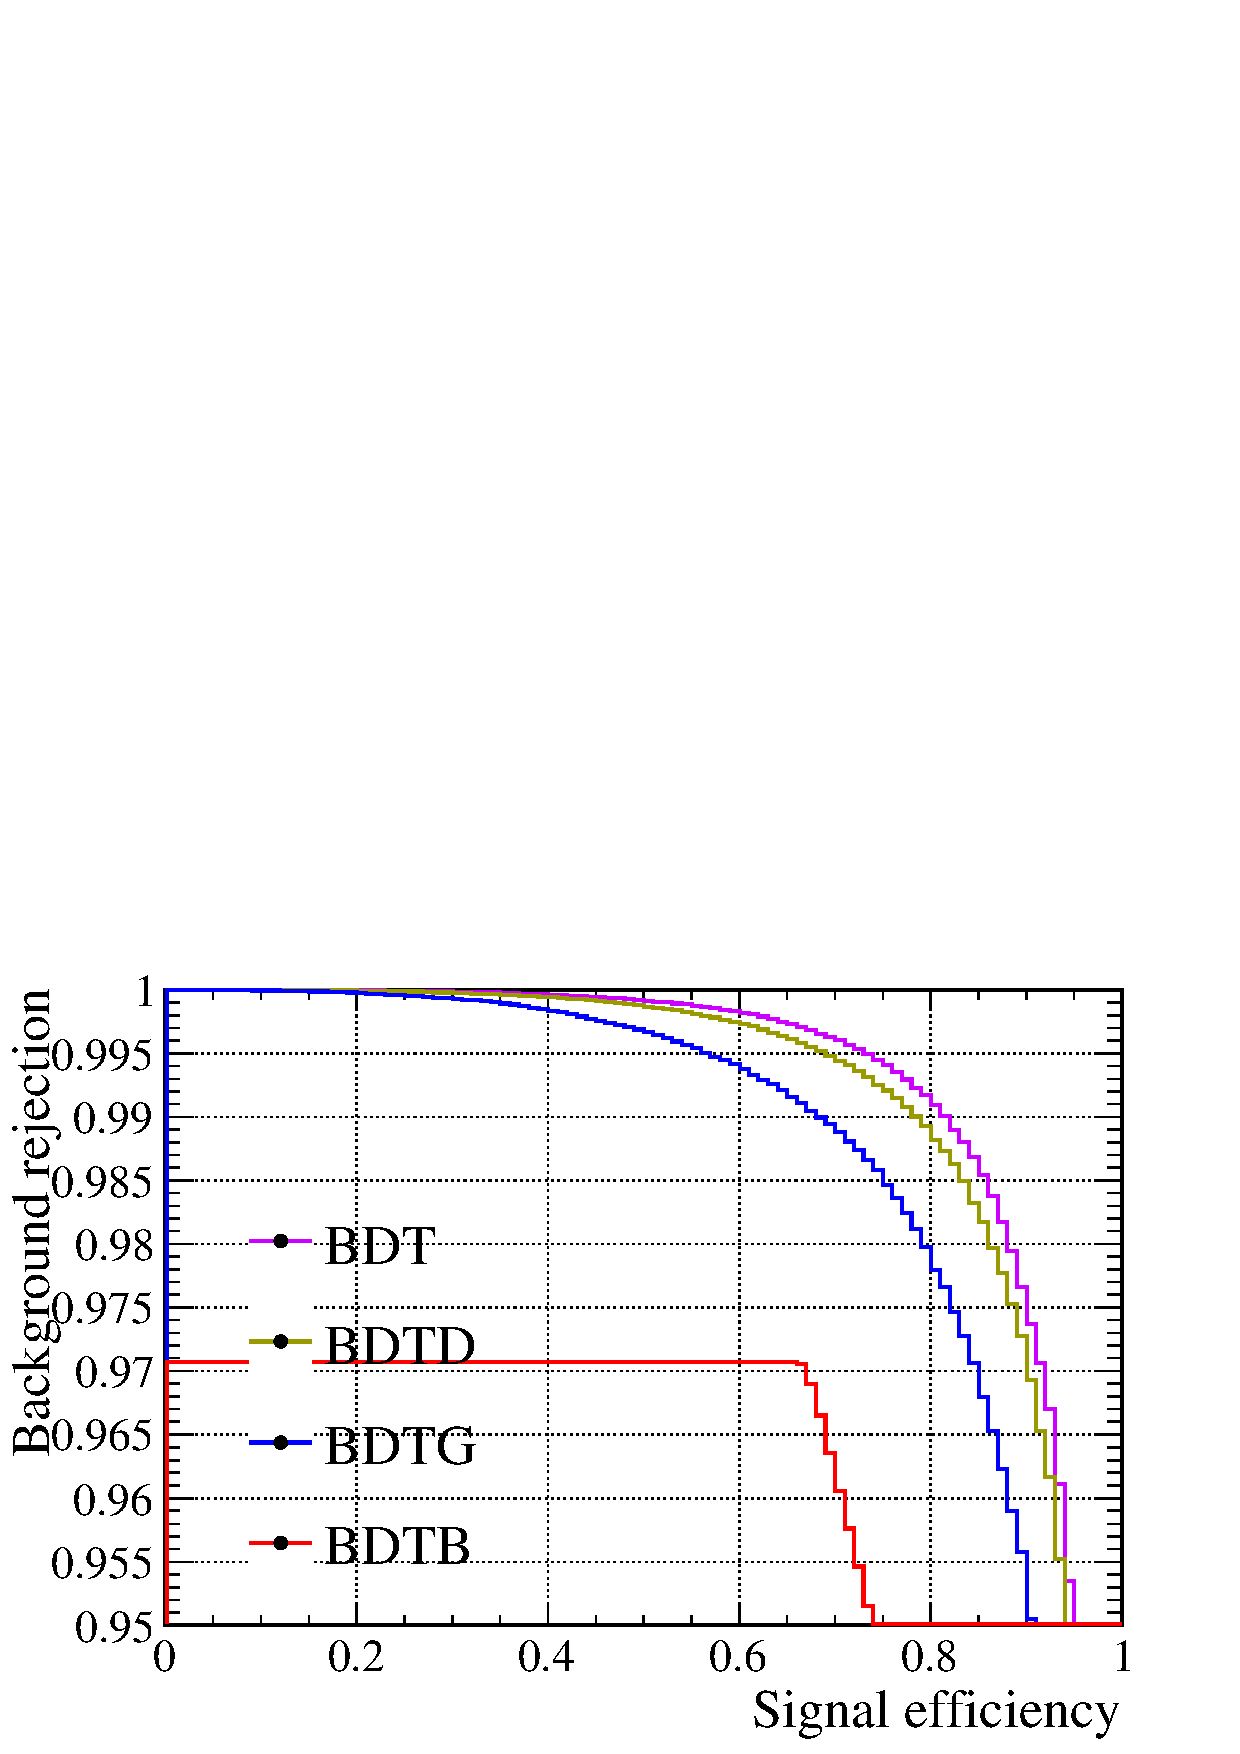
\includegraphics[scale=0.50]{figs/GL_BDT_Kspi0_pi0.pdf}
\includegraphics[scale=0.50]{figs/ROC_PARTIAL_noGhost.pdf}%GL_BDT_Kspi0_nopi0_VC.pdf}
\caption{ROC curves for the FULL (top) and PARTIAL (bottom) categories.  \label{fig:ROC}} % TODO \textcolor{red}{Resize, remove BDTB}
\end{center}

\end{figure}

%Signal and background histograms of input variables (plots for input variable distributions)
The ROC (Receiver Operating Characteristic) curves obtained for both cases are represented in \figref{fig:ROC}. 
Finally, in \figref{fig:MVAhistos_FULL1}, \figref{fig:MVAhistos_FULL2} and \figref{fig:MVAhistos_PARTIAL} the histograms for signal and background of the BDT input variable distributions are shown for the 
FULL and PARTIAL categories, respectively. 
We find that the fraction of MC signal \KS coming from $b$ or $c$ decays
is less than a per mil.

\begin{figure} [htb!]
\begin{center}
\includegraphics[scale=0.20]{figs/DOCAFULL.pdf}
\includegraphics[scale=0.20]{figs/mu1ipsFULL.pdf}
\includegraphics[scale=0.20]{figs/mu2ipsFULL.pdf}
\includegraphics[scale=0.20]{figs/PhiFULL.pdf}
\includegraphics[scale=0.20]{figs/cTh1FULL.pdf}
\includegraphics[scale=0.20]{figs/cTh2FULL.pdf}
\includegraphics[scale=0.20]{figs/K_dec_angleFULL.pdf}
\includegraphics[scale=0.20]{figs/KSipsFULL.pdf}
\includegraphics[scale=0.20]{figs/KS_ptFULL.pdf}
\includegraphics[scale=0.20]{figs/KSdissigFULL.pdf}
\includegraphics[scale=0.20]{figs/pi0massFULL.pdf}
\includegraphics[scale=0.20]{figs/XiFULL.pdf}
\includegraphics[scale=0.20]{figs/PIDmu_mu1FULL.pdf}
\includegraphics[scale=0.20]{figs/PIDmu_mu2FULL.pdf}
\includegraphics[scale=0.20]{figs/Vchi2FULL.pdf}
\includegraphics[scale=0.20]{figs/KS_IPFULL.pdf}
\includegraphics[scale=0.20]{figs/mu1_track_Chi2DoFFULL.pdf}
\includegraphics[scale=0.20]{figs/mu2_track_Chi2DoFFULL.pdf}
\includegraphics[scale=0.20]{figs/mu1_hitsInOTFULL.pdf}
\includegraphics[scale=0.20]{figs/mu2_hitsInOTFULL.pdf}
\includegraphics[scale=0.20]{figs/mu1_hitsInITFULL.pdf}
\includegraphics[scale=0.20]{figs/mu2_hitsInITFULL.pdf}
\includegraphics[scale=0.20]{figs/mu2_hitsInTTFULL.pdf}
\includegraphics[scale=0.20]{figs/mu1_hitsInTTFULL.pdf}
\caption{Input variable distributions for signal (red) and background (black) for the FULL case. \label{fig:MVAhistos_FULL1}}
\end{center}
\end{figure}

\begin{figure} [htb!]
\begin{center}
\includegraphics[scale=0.20]{figs/mu2_hitsInVFULL.pdf}
\includegraphics[scale=0.20]{figs/mu1_hitsInVFULL.pdf}
\includegraphics[scale=0.20]{figs/SV1FULL.pdf}
\includegraphics[scale=0.20]{figs/SV2FULL.pdf}
\includegraphics[scale=0.20]{figs/SV3FULL.pdf}
\caption{Input variable distributions for signal (red) and background (black) for the FULL case. \label{fig:MVAhistos_FULL2}}
\end{center}
\end{figure}

\begin{figure} [htb!]
\begin{center}
\includegraphics[scale=0.20]{figs/DOCAPARTIAL.pdf}
\includegraphics[scale=0.20]{figs/mu1ipsPARTIAL.pdf}
\includegraphics[scale=0.20]{figs/mu2ipsPARTIAL.pdf}
\includegraphics[scale=0.20]{figs/BipsPARTIAL.pdf}
\includegraphics[scale=0.20]{figs/BptPARTIAL.pdf}
\includegraphics[scale=0.20]{figs/BdissigPARTIAL.pdf}
\includegraphics[scale=0.20]{figs/PIDmu1PARTIAL.pdf}
\includegraphics[scale=0.20]{figs/PIDmu2PARTIAL.pdf}
\includegraphics[scale=0.20]{figs/Vchi2PARTIAL.pdf}
\includegraphics[scale=0.20]{figs/mu1_track_Chi2DoFPARTIAL.pdf}
\includegraphics[scale=0.20]{figs/mu2_track_Chi2DoFPARTIAL.pdf}
\includegraphics[scale=0.20]{figs/mu1_hitsInOTPARTIAL.pdf}
\includegraphics[scale=0.20]{figs/mu2_hitsInOTPARTIAL.pdf}
\includegraphics[scale=0.20]{figs/mu2_hitsInITPARTIAL.pdf}
\includegraphics[scale=0.20]{figs/mu1_hitsInITPARTIAL.pdf}
\includegraphics[scale=0.20]{figs/mu1_hitsInTTPARTIAL.pdf}
\includegraphics[scale=0.20]{figs/mu2_hitsInTTPARTIAL.pdf}
\includegraphics[scale=0.20]{figs/mu1_hitsInVPARTIAL.pdf}
\includegraphics[scale=0.20]{figs/mu2_hitsInVPARTIAL.pdf}
\includegraphics[scale=0.20]{figs/SV1PARTIAL.pdf}
\includegraphics[scale=0.20]{figs/SV2PARTIAL.pdf}
\includegraphics[scale=0.20]{figs/SV3PARTIAL.pdf}
\caption{Input variable distributions for signal (red) and background (black) for the PARTIAL case.
\label{fig:MVAhistos_PARTIAL}}
\end{center}
\end{figure}



